\section{}
\[
H(s)=\frac{10\sqrt{202}\,s}{(s+1)(s+10)}\,.
\]
\subsection{Bode-Diagramm}
\begin{center}
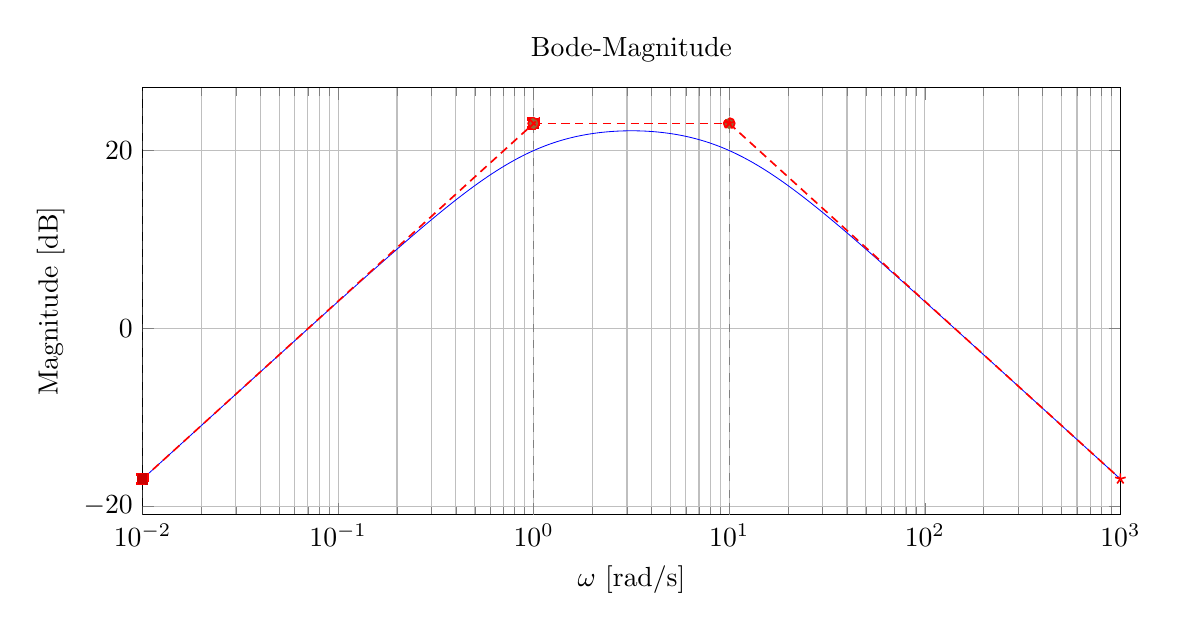
\begin{tikzpicture}
\begin{semilogxaxis}[
  width=14cm,height=7cm,
  xmin=1e-2,xmax=1e3,
  xlabel={$\omega$ [rad/s]},
  ylabel={Magnitude [dB]},
  ytick distance=20,
  grid=both,
  title={Bode-Magnitude}
]
\addplot[
  domain=1e-2:1e3,
  samples=600,
  mark=none,
  line width=0.3pt,
  blue
] {20 + 10*ln(202)/ln(10) + 20*ln(x)/ln(10) - 20*ln(sqrt(1 + x^2))/ln(10) - 20*ln(sqrt(100 + x^2))/ln(10)};
\addplot+[domain=1e-2:1,samples=2,dashed,dash pattern=on 3pt off 2pt,line width=0.6pt,red] {10*ln(202)/ln(10) + 20*ln(x)/ln(10)};
\addplot+[domain=1:1e1,samples=2,dashed,dash pattern=on 3pt off 2pt,line width=0.6pt,red] {10*ln(202)/ln(10)};
\addplot+[domain=1e1:1e3,samples=2,dashed,dash pattern=on 3pt off 2pt,line width=0.6pt,red] {10*ln(202)/ln(10) - 20*ln(x/10)/ln(10)};
\draw[gray,dashed] (rel axis cs:0,0) -- (rel axis cs:0,1);
\draw[gray,dashed] (axis cs:1,\pgfkeysvalueof{/pgfplots/ymin}) -- (axis cs:1,\pgfkeysvalueof{/pgfplots/ymax});
\draw[gray,dashed] (axis cs:10,\pgfkeysvalueof{/pgfplots/ymin}) -- (axis cs:10,\pgfkeysvalueof{/pgfplots/ymax});
\node[gray,anchor=south east] at (axis cs:1,\pgfkeysvalueof{/pgfplots/ymax}) {\scriptsize Pol $\omega_{p1}=1$};
\node[gray,anchor=south east] at (axis cs:10,\pgfkeysvalueof{/pgfplots/ymax}) {\scriptsize Pol $\omega_{p2}=10$};
\end{semilogxaxis}
\end{tikzpicture}
\vspace{6mm}
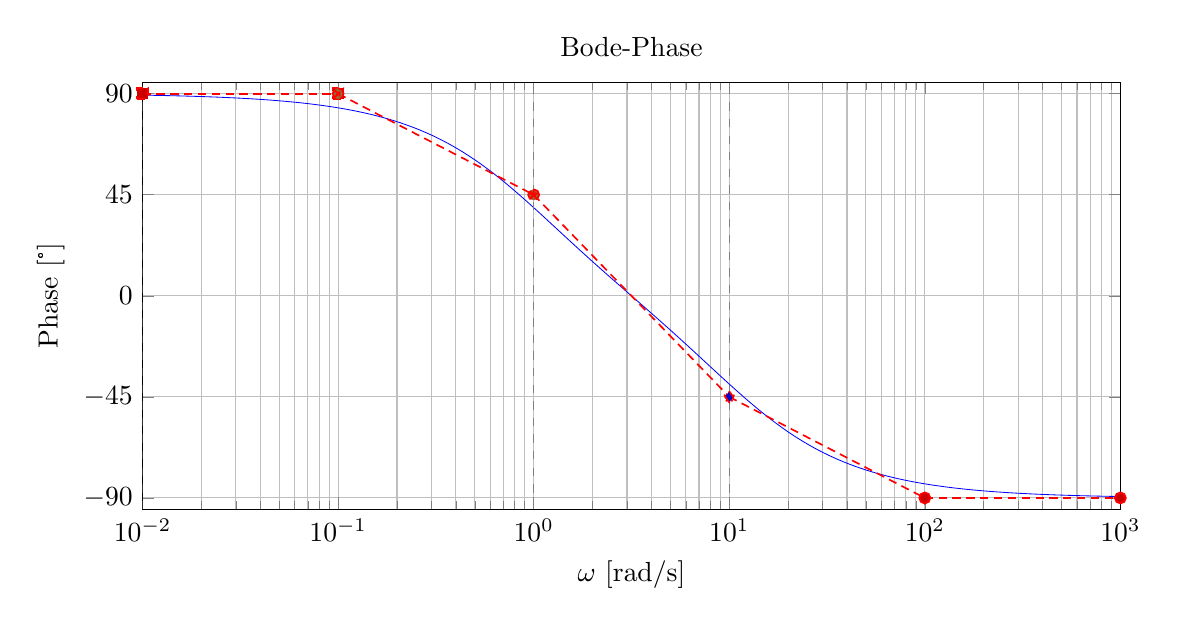
\begin{tikzpicture}
\begin{semilogxaxis}[
  width=14cm,height=7cm,
  xmin=1e-2,xmax=1e3,
  ymin=-95,ymax=95,
  ytick distance=45,
  xlabel={$\omega$ [rad/s]},
  ylabel={Phase [°]},
  grid=both,
  title={Bode-Phase}
]
\addplot[
  domain=1e-2:1e3,
  samples=600,
  mark=none,
  line width=0.3pt,
  blue
] {90 - atan(x) - atan(x/10)};
\addplot+[domain=1e-2:1e-1,samples=2,dashed,dash pattern=on 3pt off 2pt,line width=0.6pt,red] {90};
\addplot+[domain=1e-1:1e0,samples=2,dashed,dash pattern=on 3pt off 2pt,line width=0.6pt,red] {45 - 45*ln(x)/ln(10)};
\addplot+[domain=1e0:1e1,samples=2,dashed,dash pattern=on 3pt off 2pt,line width=0.6pt,red]{45 - 90*ln(x)/ln(10)};
\addplot+[domain=1e1:1e2,samples=2,dashed,dash pattern=on 3pt off 2pt,line width=0.6pt,red]{-45 - 45*ln(x/10)/ln(10)}; % bei 10: -45°, bei 100: -90°

\addplot+[domain=1e2:1e3,samples=2,dashed,dash pattern=on 3pt off 2pt,line width=0.6pt,red] {-90};
\draw[gray,dashed] (rel axis cs:0,0) -- (rel axis cs:0,1);
\draw[gray,dashed] (axis cs:1,\pgfkeysvalueof{/pgfplots/ymin}) -- (axis cs:1,\pgfkeysvalueof{/pgfplots/ymax});
\draw[gray,dashed] (axis cs:10,\pgfkeysvalueof{/pgfplots/ymin}) -- (axis cs:10,\pgfkeysvalueof{/pgfplots/ymax});
\node[gray,anchor=south east] at (axis cs:1,\pgfkeysvalueof{/pgfplots/ymax}) {\scriptsize Pol $\omega_{p1}=1$};
\node[gray,anchor=south east] at (axis cs:10,\pgfkeysvalueof{/pgfplots/ymax}) {\scriptsize Pol $\omega_{p2}=10$};
\end{semilogxaxis}
\end{tikzpicture}
\end{center}
\newpage
\subsection{Erklärung (ausführlich)}
\begin{description}[leftmargin=1.2em,labelsep=.6em,font=\bfseries]

\item[1. Normalform herstellen.]
\[
H(s)=\frac{10\sqrt{202}\,s}{(s+1)(s+10)}
= K_0\cdot s^{\,r}\cdot \frac{1}{(1+sT_{p1})(1+sT_{p2})}
\]
mit
\[
K_0=\sqrt{202},\quad r=1,\quad T_{p1}=1,\quad T_{p2}=\tfrac{1}{10}.
\]
\[
\underline{F}_1(s)=\frac{1}{1+sT_{p1}}=\frac{1}{1+s},\qquad
\underline{F}_2(s)=\frac{1}{1+sT_{p2}}=\frac{1}{1+\tfrac{s}{10}}
\]

\item[2. Eckfrequenzen bestimmen und sortieren.]
\[
\omega_{p1}=\frac{1}{T_{p1}}=1\,\mathrm{rad/s},\qquad
\omega_{p2}=\frac{1}{T_{p2}}=10\,\mathrm{rad/s},\qquad
\omega_{p1}<\omega_{p2}.
\]

\item[3. Startpunkt des Amplitudengangs festlegen (Geradennäherung).]
Setze \(\omega_{\min}=\omega_{p1}=1\).
\[
F_{\mathrm{dB}}(\omega_{\min})
=20\log_{10}\!\Big(|K_0\underline{F}_{ges}^*(0)|\,\omega_{\min}^{\,r}\Big)
=20\log_{10}(\sqrt{202}\cdot 1) \approx 23\,\mathrm{dB}.
\]
Ankerpunkt: \(23\,\mathrm{dB}\) bei \(\omega=1\).

\item[4. Verlauf links vom Startpunkt zeichnen.]
Für \(\omega<1\): Anfangssteigung \(r\cdot 20=+20\,\mathrm{dB/dec}\). Zeichne links vom Startpunkt die Gerade mit \(+20\,\mathrm{dB/dec}\) durch den Ankerpunkt.

\item[5. Steigungswechsel an den Eckfrequenzen eintragen.]
Pol bei \(\omega_{p1}=1\): Steigungsänderung \(-20\,\mathrm{dB/dec}\) \(\Rightarrow\) Netto \(0\,\mathrm{dB/dec}\) in \([1,10]\) (betragsflach).
Pol bei \(\omega_{p2}=10\): weitere \(-20\,\mathrm{dB/dec}\) \(\Rightarrow\) Netto \(-20\,\mathrm{dB/dec}\) für \(\omega\gg10\).
Geradennäherung:
\[
|H(j\omega)|_{\mathrm{dB}}\approx
\begin{cases}
10\log_{10}202+20\log_{10}\omega,& \omega\le 1,\\
10\log_{10}202,& 1<\omega\le 10,\\
10\log_{10}202-20\log_{10}(\omega/10),& \omega\ge 10.
\end{cases}
\]

\item[6. Eckabrundungen korrekt berücksichtigen.]
Jeder einfache Pol: \(-3\,\mathrm{dB}\) unter der Geradennäherung am Knick.
\[
|H(j1)|_{\mathrm{dB}}\approx 10\log_{10}202-3\ \mathrm{dB}\ \ (\approx 20\,\mathrm{dB}),\]\[
|H(j10)|_{\mathrm{dB}}\approx 10\log_{10}202-3\ \mathrm{dB}\ \ (\approx 20\,\mathrm{dB}).
\]

\item[7. Phasenstartwert festlegen.]
Verwende die Regel für $K_0\underline{F}_{ges}^*(0) > 0$
\[
\varphi(0)= r\cdot 90^\circ = 1\cdot 90^\circ = +90^\circ.
\]

\item[8. Phasenänderung durch die Polglieder eintragen.]
Nullstelle im Ursprung liefert konstant \(+90^\circ\). Pol bei \(1\): \(-90^\circ\) über \([0.1,10]\). Pol bei \(10\): \(-90^\circ\) über \([1,100]\). In \([1,10]\) überlappen sich beide Polbeiträge und addieren sich (Netto-Steilheit = Summe der Einzelsteilheiten). Näherung:
\[
\varphi(\omega)\approx
\begin{cases}
+90^\circ,& \omega\le 0.1,\\
45^\circ-45^\circ\log_{10}\omega + 90^\circ,& 0.1<\omega<1,\\
45^\circ-90^\circ\log_{10}\omega + 90^\circ,& 1<\omega<10,\\
-45^\circ-45^\circ\log_{10}(\omega/10),& 10<\omega<100,\\
-90^\circ,& \omega\ge 100.
\end{cases}
\]
(vereinfacht im Plot als \(90- \arctan\omega - \arctan(\omega/10)\) gezeigt; Grenzwert \(\varphi(\infty)=-90^\circ\)).

\item[9. Grenzwerte und Konsistenz prüfen.]
DC: \(|H(0)|=0\Rightarrow -\infty\,\mathrm{dB}\), \(\varphi(0)=+90^\circ\).
HF: \(|H(j\omega)|\sim \sqrt{202}\,\frac{\omega}{\omega^2/10}= \sqrt{202}\cdot \frac{10}{\omega}\Rightarrow 10\log_{10}202-20\log_{10}(\omega/10)\,\mathrm{dB}\), \(\varphi(\infty)=+90^\circ-180^\circ=-90^\circ\).
Pol-/Nullzählung: \(m=1\), \(n=2\Rightarrow (m-n)\cdot 90^\circ=-90^\circ\) konsistent.

\end{description}

\subsubsection*{Stückweise Näherungen (für die Skizze)}
\[
|H(j\omega)|_{\mathrm{dB}}\approx
\begin{cases}
10\log_{10}202+20\log_{10}\omega,& \omega\ll 1,\\[2pt]
10\log_{10}202-3,& \omega=1,\\[2pt]
10\log_{10}202,& 1\ll\omega\ll 10,\\[2pt]
10\log_{10}202-3,& \omega=10,\\[2pt]
10\log_{10}202-20\log_{10}(\omega/10),& \omega\gg 10,
\end{cases}
\]\[
\varphi(\omega)\approx
\begin{cases}
+90^\circ,& \omega\le 0.1,\\[2pt]
45^\circ-45^\circ\log_{10}\omega + 90^\circ,& 0.1<\omega<1,\\[2pt]
45^\circ-90^\circ\log_{10}\omega + 90^\circ,& 1<\omega<10,\\[2pt]
-45^\circ-45^\circ\log_{10}(\omega/10),& 10<\omega<100,\\[2pt]
-90^\circ,& \omega\ge 100.
\end{cases}
\]

\newpage